%\usepackage[top=0.5cm,bottom=0.5cm,left=0.5cm,right=0.5cm]{geometry}
%\usepackage[a5paper,top=0cm,bottom=0cm,left=0cm,right=0cm]{geometry}
\documentclass{article}
\usepackage{listings}
\usepackage{color} %red, green, blue, yellow, cyan, magenta, black, white
\definecolor{mygreen}{RGB}{28,172,0} % color values Red, Green, Blue
\definecolor{mylilas}{RGB}{170,55,241}
\usepackage[swedish,english]{babel}
\usepackage[utf8]{inputenc}
\usepackage{amsmath}
\usepackage{graphicx}
\usepackage{float}
\usepackage{hyperref}
\usepackage{caption}
\usepackage{lipsum}
\usepackage{listings}
\usepackage{listingsutf8}
\usepackage{xcolor}
\usepackage{textcomp}
\usepackage{units}
\usepackage{bbm}
\usepackage{url}
\usepackage[english]{isodate}
\usepackage{gensymb}
\usepackage{amssymb}
\usepackage{amsthm}
\usepackage{fullpage}
\usepackage{tikz}
\usepackage{pgfplots} 
\usepackage{pgfgantt}
\usepackage{pdflscape}
\pgfplotsset{compat=newest} 
\pgfplotsset{plot coordinates/math parser=false}
\usepackage{todonotes}
\usepackage{siunitx}
\usepackage{geometry}
\usepackage[utf8]{inputenc}
\usepackage[T1]{fontenc}
\usepackage[english,swedish]{babel}
\usepackage{csquotes}
\usepackage{amsmath}
\usepackage{ae} 
\usepackage{units}
\usepackage[version=4]{mhchem}
\usepackage{icomma}
\usepackage{color}
\usepackage{graphicx}
\usepackage{bbm}
\usepackage{textcomp}
\usepackage{hyperref}
\usepackage{verbatim}
\usepackage{wrapfig}
%\usepackage{natbib}
\usepackage{multirow}
\usepackage{subfig}
\usepackage[titletoc]{appendix}
\usepackage{float}
\usepackage{parskip}
\usepackage{subfiles}
\newcommand{\HRule}{\rule{\linewidth}{0.5mm}}
\usepackage{chemfig} %https://en.wikibooks.org/wiki/LaTeX/Chemical_Graphics
\usepackage[
backend=biber,
style=ieee,
citestyle=numeric 
]{biblatex}
%https://www.tablesgenerator.com/
%https://www.codecogs.com/latex/eqneditor.php
\addbibresource{references.bib}
\addbibresource{timmie.bib}
 % här ligger även bra hemsidor som man kan använda
\begin{document}

\begin{titlepage}
\begin{centering}

{\huge\bfseries Vanadinutvinning från LD slagg som använts som syrebärare i förbränningsprocesser \par}
\vspace{1cm}
{\scshape\Large Projektsplanering \textbf{}\par}
{\scshape\Large \par}
{\Large\itshape Victor Hernvall, Frida Tropp,  \\ Timmie Dzafo Paulsson, Marcus Mellqvist \\ Stefan Ewaldsson, och Marcus Thim.\par}
{\large \today\par}

{   \par}
{   \par}
{    \par}


\begin{figure}[!ht]
\centering

\includegraphics[scale=0.3]{chalmers.png}
\label{fig:chalmers}

\end{figure}
\centering{\textbf{CHALMERS TEKNISKA HÖGSKOLA} \par}


\end{centering}
\end{titlepage}

\newpage 
\thispagestyle{empty}
\pagenumbering{roman}
\setcounter{page}{3}
\hspace{0pt}
\vfill
\begin{centering}
\Large Stort tack till Fredrik Hildor, Duygu Yilmaz, och Henrick Leion.
\vfill
\end{centering}
\hspace{0pt}
\begin{centering}
\topskip15pt
\end{centering}
\newpage
\thispagestyle{empty}
\thispagestyle{empty}
\tableofcontents
\thispagestyle{empty}
\newpage
\pagenumbering{arabic}
\section{Bakgrund}

\section{Syfte}

\section{Metod}

Laborationerna kommer i största utsträckningen ske i grupper av två och två, utan att ha någon säkerlid indelning av personer. Utan det kommer snarare bero på vilka gruppmedlemmar som är tillgängliga. I början av varje vecka kommer ett möte att hållas för att planera den kommande veckan och se vad som gjordes föregående vecka. 

Valet av metod grundar sig i tidigare uppställningar för liknande laborationer, samt en laborations uppställning som visas av handledaren Duygu Yilmaz\cite{Aarabi-Karasgani2010}. 

\begin{table}[H]
\label{metodtab}
\caption{Premilinär test uppställning.}
\begin{tabular}{|l|c|c|c|}
\hline
\textbf{\begin{tabular}[c]{@{}l@{}}Influencerande \\ faktorer\end{tabular}}              & \multicolumn{1}{l|}{\textbf{\begin{tabular}[c]{@{}l@{}}H$_{2}$SO$_{4}$ \\ koncentration [M]\end{tabular}}} & \multicolumn{1}{l|}{\textbf{\begin{tabular}[c]{@{}l@{}}Ratio mellan fast \\ och flytande [ml/g]\end{tabular}}} & \multicolumn{1}{l|}{\textbf{\begin{tabular}[c]{@{}l@{}}Laknings\\ Temperatur  [$\degree$C]\end{tabular}}} \\ \hline
\textbf{\begin{tabular}[c]{@{}l@{}}H$_{2}$SO$_{4}$ \\ koncentration [M]\end{tabular}}    & 1,2,3,4                                                                                                    & 6:1                                                                                                           & 70                                                                                                        \\ \hline
\textbf{\begin{tabular}[c]{@{}l@{}}Ratio mellan fast\\ och flytande [ml/g]\end{tabular}} & 3                                                                                                          & 2:1, 4:1, 6:1, 8:1                                                                                            & 70                                                                                                        \\ \hline
\textbf{\begin{tabular}[c]{@{}l@{}}Laknings \\ Temperatur  [$\degree$C]\end{tabular}}    & 3                                                                                                          & 6:1                                                                                                           & 60,70,80,90                                                                                               \\ \hline
\end{tabular}
\end{table}


Metoden kommer att valideras genom att analysera proverna med en rad olika metoder. Atomabsorptionsspektroskopi, AAS, och röntgenkristallografi, XRD från engelska X-ray diffraction, och svepelektronmikroskop, SEM. De olika metoderna används för att validera olika delar av arbetet. AAS används för att validera att vi har lyckats laka ur vanadinet ur LD slagget. XRD kommer att användas för att analysera kristallstrukturen av LD slagget för och efter att det har rostats och vid olika intervaller under rostningen för att se sammansättningen av de olika ämnena i krisallen. Slutligen så kommer SEM användas för att se var i LD slagget som de olika ämnena befinner sig i slagg partiklarna. 

Planeringen är att en literaturstudie ska ske parallellt med laborationerna för att kunna ge möjlighet till djupare inlärning och förklaring av ämnet. Det innebär användnings områden av vanadin, användadet av LD slagg och dess deponering i nuläget. Även vilka fördelar och nackdelar med processen och vad det kan göra för samhällsnytta inför i framtiden. 

\section{Problem} 
Den huvudsakliga uppgiften består av att jämföra möjligheterna att utvinna vanadin ur LD-slagg som har genomgått olika behandlingar. Extraktionen sker genom lakning.

Deluppgift ett kommer bestå i att utföra en rad experiment som undersöker i vilket medium och under vilka förhållanden lakningen är mest gynnsam.

Deluppgift två kommer vara att jämföra resultaten av utvinning av vanadin från LD-slagg som är obearbetat och de som använts som syrebärare.

Utöver de test som kommer göras för att analysera mängden utvunnen vanadin kommer det även testas vilken halt fosfor som erhålls i samma prov.
I mån av tid kan det även testas specifikt för fosfor och även ändra lakningsparametrar för att underlätta utvinningen av fosfor.
\section{Avgränsningar}
Även om det är ett ämnes område som det i nuläget redan görs forskning på, inom olika applikationer och djupare förståelse, så finns det mycket potential i det här projektet. Men det med begränsade resurser, främst tid, så kommer vi behöva göra en mängd avgränsningar på vad som kommer att kollas på. 


\section{Samhälleliga och etiska aspekter}
Det finns en  väldigt stor industri som tillämpar LD-processen för att tillverkar stål. Till följd av detta finns även en väldigt stor sidoström innehållande stålslagg, kallat LD-slagg. Detta slagg läggs i nuläget på deponi, vilket skulle kunna vara en negativ samhällelig aspekt om det hanteras illa. Det vill säga att deponin läggs på ett ställe där den blir skrymmande eller stör utsikten. 

En mer etisk aspekt av deponin vore i fallet att exempelvis tungmetaller och fosfor läcker ut i närliggande vattendrag eller jordmån.

Genom att använda LD-slagg som syrebärare i förbränningsprocesser och vidare laka den brända slaggen för utvinning av vanadin ger en hållbar och cyklisk process som utnyttjar restprodukter från en annan process som är lättillgänglig och finns i stora kvantiteter.
\section{Tidsplan}


\printbibliography
\appendix
\section{Appendix}
\begin{figure}[H]
    \centering
    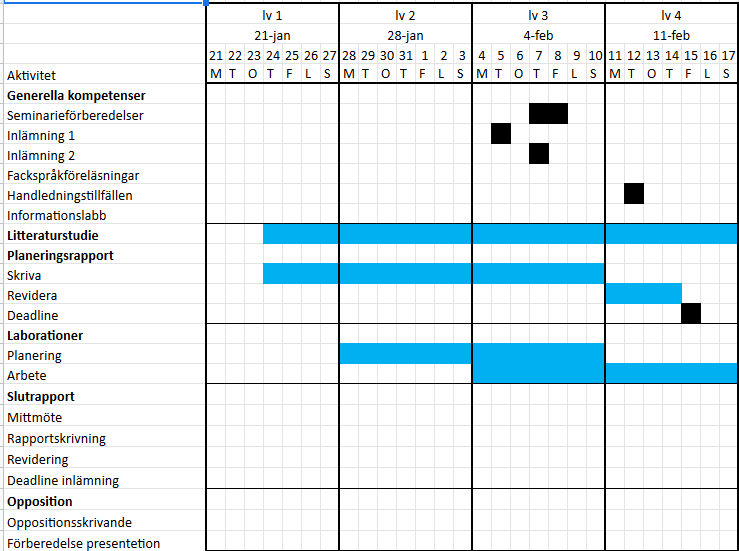
\includegraphics[scale=0.7]{Gantt.PNG}
    \caption{Gantt-schema över veckorna relaterat till projektbeskrivningen}
    \label{fig:Gantt}
\end{figure}
\end{document}

